\documentclass[12pt]{report}

\usepackage[utf8]{inputenc}   
\usepackage[top=2cm, bottom=2cm, left=2cm, right=2cm]{geometry}
\usepackage{color}
\usepackage{array}
\usepackage[T1]{fontenc}
\usepackage{hyperref}
\usepackage{graphicx}
\usepackage { boxedminipage }


\begin{document}

\begin{minipage}{0.3\linewidth}
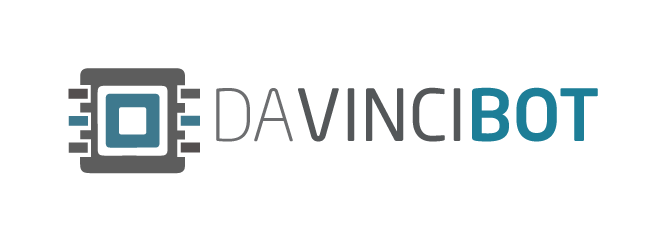
\includegraphics[scale = 0.2]{img/logo_assos.png}
\end{minipage}
\vspace{1cm}
% PAS TOUCHER AU DESSUS !!! 


% modifier numéro compte rendu et numéro de semaine

\begin{center}
\textbf{Script de la vidéo de lancement}
\end{center}

\textbf{Chargés du script : Théo Isambourg, Nicolas Fontaine, Guillaume Fradet}

\vspace{1cm}

Nous sommes DaVinciBot, l'association robotique du pôle universitaire Leonard de Vinci. 
\\Nous concourons pour la troisième année consécutive à la coupe de France de robotique qui  se déroulera à la  Roche sur Yon du 25 au 27 mai 2017.
\\Pour participer à ce concours, nous avons monté un groupe de 14 étudiants de l'ESILV actuellement en 2ème et 3ème année.
\\Cinq d'entre nous ont déjà vécu cette aventure l'année dernière, ils apporteront donc leurs expériences; tandis que les autres introduiront des idées nouvelles pour répondre au nouveau challenge de cette année. 
\\La coupe de France de robotique est un événement qui rassemble plus de 200 jeunes équipes amateurs, qui doivent créer leur robot suivant un cahier des charges bien précis. Ils s'affrontent ensuite sous forme de duel sur une grande table (image table).
\\Cette année le thème de la compétition est la lune (image Moon Village de la CFR). Les robots devront donc réaliser divers actions rapportant plus ou moins de points comme : construire  une base lunaire, récolter des échantillons de minerais et roches présents sur la table, et lancer une petite fusée dans les 5 dernières secondes du match. L'équipe ayant rapportée le maximum de points gagne le duel.
\\Afin d'effectuer toutes ces tâches, nous allons utiliser plusieurs outils et technologies innovantes tels que ROS, Robot Operating System, qui installé sur notre Raspberry Pi2 pourra contrôler simultanément toutes nos cartes Arduino, afin d'avoir un robot multitâche. Nous  utiliserons le logiciel Solidworks pour modéliser nos pièces, que nous imprimerons ensuite en 3D au FabLab de notre école. Et nous utiliserons les langages C et Python pour toute la partie programmation. Aussi,afin de travailler sur un répertoire commun, nous utiliserons GitHub, un logiciel de gestion de version.
\\(break)
\\Notre objectif cette année est d'atteindre le top 50 ! 
\\Suivez notre aventure sur la page facebook DaVinciBot, et sur notre site web. 
\\Rendez-vous en mai pour la compétition !




\end{document}